%\documentclass[a4paper,10pt]{report}
\documentclass[conference]{IEEEtran}
\usepackage[utf8]{inputenc}

% Usepackages, could be moved to a new file
% Long Table and decimal aligned columns
\usepackage{dcolumn}
\usepackage{longtable}

% Mathematics support
\usepackage{amsmath}
\usepackage{amsthm}
\usepackage{amssymb}


% Text Control
\usepackage{xspace}
\usepackage{textcase}
\usepackage{url}%hyperref}

% Graphics
\usepackage{wasysym}
\usepackage{graphics}
\usepackage{graphicx}   % A package to allow insertion of
                        % external image files
\usepackage{epstopdf}
% Comments
\usepackage{comment}
% Citation
%\usepackage{natbib}


\newif\ifrev
% comment out the following line after the revision is proved
%\revtrue
\ifrev
  \usepackage{color}
  \usepackage[normalem]{ulem}
  \newcommand{\add}[1]{\textcolor{blue}{\uline{#1}}}
  \newcommand{\del}[1]{\textcolor{red}{\sout{#1}}}
\else
  \newcommand{\add}[1]{#1}
  \newcommand{\del}[1]{}
\fi

% Title Page
% \title{Design and Implementation for a Peer-to-peer-based Mobile VoIP
% Application}
% \title{ThinkTogether: A Collaborative App based on a Peer-to-Peer
% Infrastructure}

\title{Exploring Peer-to-Peer Infrastructure for Computer Supported
Collaborative Work Applications}

\author{\qquad Tianming Wei \qquad Yongjun Xu \qquad Yiyun Zhao \qquad Nishant Khanna \qquad Bing Gao \qquad Yvonne Coady\\
Department of Computer Science\\
University of Victoria, Victoria, BC, Canada\\}


\begin{document}
\maketitle
\pagestyle{plain}

\begin{abstract}
\begin{comment}
With the enhancement in technology every day there are so many applications
being developed every day. There are a lot of applications that have been
developed to record presentations and to upload content onto the server for
later reference. ThinkTogether is much more than that. Not only does it support
basic functions like giving presentation, and adding comments and marking
important points, ThinkTogether also provides multilayer function, which achieve
better performance by separating different users into multiple layers. As fully
functionable as the app already is, we still want to take it to the next level.
In this study, we propose a network mechanism using VoIP technology, to
introduce voice streaming feature into existing application developed by Two
Tall Totems.
\end{comment}
Computer Supported Collaborative Work (CSCW) has been greatly enhanced by
technology that provides almost real-time capture, replay, and sharing of
content. “The cloud” has popularized ease of deployment for apps serviced
through a centralized approach. In this work we propose a more aggressive
design, decentralizing the location of shared content within a peer-to-peer
structure. Ease of deployment is maintained through a novel architecture for a
multilayer distributed cloud. This paper describes how this approach has shown
promise in a prototype app, {\em ThinkTogether},
and the potential to enable a consistent user experience, even for remote peers
sharing VoIP.

\end{abstract}

\begin{IEEEkeywords}
  Voice over IP, Peer-to-peer, Quality of service, Traffic balance, Bandwidth
utilization.
\end{IEEEkeywords}

%\section{Introduction}
\section{Introduction}

\begin{comment}
ThinkTogether is a mobile collaboration platform developed by Two Tall Totems, which is also a creative Bring Your Own Device (BYOD) solution. It enables teachers and students to cooperate together through the lecture in a class or presenters and attendees to participate together in a conference. The current implementation of the project on iOS supports the most functionality of the presentation, yet not with voice stream. It is essential to support the voice stream in the application for remote education since students will be able to have a better interaction with the class even if they are not in the classroom. We are going to design and implement a Peer-to-Peer (P2P) based Voice over IP (VoIP) system on the top of the existing application on iOS so that the users not only could actively enjoy the presentation on live but also could store and replay it later on the cloud.

Due to a variety of factors that could affect the quality of service (QoS) for the application, such as limited bandwidth, high volume traffic, network delay and effect of peer signal, we are going to explore and analyze a better solution with optimized performance. This project aims to create a new education model and subvert the traditional way of learning, sharing and communicating with mobile devices through different cutting-edge mobile technology. First of all, we will model a hierarchical architecture, and verify the model as well as the design with a simulation software Omnet++. After that, analysis will be applied to the data collected from the results of the simulation and we are going to discover the bottleneck in our VoIP solution as well as make an improvement.

Therefore, we propose to experiment the method of pushing data among all the 
devices and ensure the usage of bandwidth that is enough for each user as well 
as for the cloud server. We are going to implement a stable service based on 
Voice over IP (VoIP), Peer-to-peer (P2P) or Multi-peer technology, which would 
also be scalable for large amount users with mobile devices in the existing App. 
With our partner Two Tall Totems, development on this project with these 
advanced communication and network technology could greatly change how people 
think together and help to build a better world.
\end{comment}

%background
Collaboration platforms for Computer Supported Collaborative Work (CSCW) enable 
users to leverage technology to cooperatively develop shared content.   
Successful platforms now support everything from education to medicine, 
typically supported through a centralized service or cloud. Though read-only 
content distribution has been successfully shared between 
peers~\cite{XG_P2P_INFO04}, mutable content with complex interactions and 
dependencies 
has been more difficult to decentralize. Essentially, the problem is that 
decentralized approaches require coordination as nodes can come and go, and 
connections can fail, creating a myriad of different failure modes.

%problem
In this paper, we overview the design of a Peer-to-Peer (P2P) infrastructure for 
a CSCW application, ThinkTogether.  ThinkTogether is an iOS prototype for 
creating and sharing content in almost real-time. We consider the specific 
problem of Voice over IP (VoIP), as it is representative of a stream of content 
that is particularly sensitive to service disruptions.  Our goal is to be able 
to share all content, including voice, live, but also allow users to replay it 
later based on access to a shared server or the cloud.   Due to the variety of 
factors that could affect the quality of service (QoS) for the application, such 
as limited bandwidth, high volume traffic, network delay and the effects of 
other peers, we propose a dynamically decentralized approach, in order to 
optimize the network performance as conditions change in the system.  We 
consider this 
in a case study for an educational platform, which could ultimately subvert the 
traditional way of learning, sharing and communicating with mobile technology.
 

%section description
This paper is organized as follows.  After an overview of related work (Section 
II), we present our model of a hierarchical architecture, and provide the 
verification of the model (Section III) as well as the design with simulation 
software Omnet++~\cite{A_OMNET_ESM01}. We then describe the ways in which 
the simulation results inform the implementation of the system.  
In particular, we identify bottlenecks to anticipate in the VoIP educational 
platform case study. The analysis underscores the importance of augmenting the 
existing prototype with a means of easily distributing data throughout the peers 
in the system, in a way that provides adequate bandwidth for both the current 
users and the cloud-based content capture (Section IV).  We generalize this 
construct, and propose that if we treat the platform as a {\em distributed 
cloud}, it may be able to address the key challenge---to scale across 
potentially thousands of mobile devices, all creating and modifying shared 
content, in a globally distributed system (Section V).  We conclude with an 
outline of future work (Section VI).

\begin{comment}
This paper is organized as follows.  We first present our model of a 
hierarchical architecture, and provide the verification of the model as well as 
the design with simulation software Omnet++~\cite{CITATION} (Section 1). We then 
describe the ways in which the simulation results inform the implementation of 
the system (Section 2).  In particular, we identify bottlenecks to anticipate in 
the VoIP educational platform case study.  The analysis underscores the 
importance to augment the existing prototype with a means of easily distributing 
data throughout the peers in the system, in a way that provides adequate 
bandwidth for both the current users and the cloud-based content capture 
(Section 3).  We generalize this construct, and propose that if we treat the 
platform as a {\em distributed cloud}, it may be able to address the key 
challenge---to scale across potentially thousands of mobile devices, all 
creating and modifying shared content, in a globally distributed system (Section 
4).  We conclude with an outline of future work (Section 5).
\end{comment}

%\section{Related Work}\label{simu}
\section{Related Work}

\begin{comment}
Voice over IP (VoIP):

There are various studies that have been done in the field of VoIP (Voice
over IP) which is a technology used
for voice communication over multimedia devices with the help of the IP
protocols. Some of the related work has been done by Wook \& Kang [1] where
their main focus is based on VoIP using SIP( Session Initiation Protocol) for
smartphones working on iOS, Android \& Windows based OS , In our project we’ll
be using a similar technology of VoIP but our focus is on iOS devices i.e.
mostly IPAD’s. Similarly there is some other research done by Fathi et al. [2]
for the optimization of VoIP services in Wireless networks and how to reduce the
disruptions in real-time sessions by focusing on the network layer and not so
much on the link layer, In our project we aim to use a similar concept where we
aim to reduce delay in voice streaming for live presentations for Wireless
devices with a focus on both the network and link layer. Work done by Rao et al.
[3] is based on providing VoIP services for GSM based devices without making any
modifications in the GSM network, we use a similar concept for providing VoIP
services but with a focus on iOS devices instead of GSM devices .
There is some work done to improve the VoIP capacity in Wireless networks done
by Fong et al. [4], we plan to use a similar concept as presented in the paper
[4] to handle voice traffic as with the voice streams during a live presentation
there is a chance that the voice traffic might increase and it is very important
to handle this traffic in the best possible way to avoid any disruption in voice
streaming in real-time. All these studies talk about VoIP applications and how
to improve the capacity of such systems in Wireless networks.
Now there some research done for VoIP in mobile devices like: Aggregation of
VoIP streams done by Komolafe \& Gardner [5], we focus on using a similar
concept but instead of aggregation of calls we are concerned with aggregation of
voice streams.
The work done by Agarwal et al. [6] is based on energy management of VoIP over
Wi-Fi for Smartphones, In our project instead of focusing on Smartphones we
focus on iOS devices (IPAD’s) , but we also use a similar concept for energy
management of VoIP over the devices and with increasing amount voice streaming
over the network the energy of the device needs to be managed in an efficient
and environment friendly manner.  Quality Measurement of VoIP over mobile
devices by Chen et al. [7] gives some methods to measure the Quality of VoIP
over mobile devices, we plan to use a similar concept as voice quality is one
the most important aspects in our project, so we need to ensure that voice
quality is perfect without any kind of noise or disruption in voice streaming
over the network. Performance Measurement of VoIP over the mobile networks by
Kim et al. [8] provide some methods to measure the performance of VoIP, we will
be using a similar approach as proposed in the paper [8] to measure the
performance of VoIP over the mobile networks and by using the results of
performance measurement we would analyse the network and try to improve any
possible disruption that might cause any kind of delay in streaming voices over
the network.
There are some other models where VoIP has been implemented using P2P
(Peer-to-peer) like: Improving performance of P2P based VoIP applications by
Wang et al. [11] where they analysed the delay in the Chinese internet system.
To analyse the delay different methods were used in the paper [11], we aim to
use a similar kind of technique to analyse the delay of voice streaming in our
application.


Skype:
There are some existing technologies that use the VoIP feature like Skype. Lot
of research has been done in this field like, An experimental study on Skype
P2P VoIP Systems done by Guha \& Daswani [12] where they study different
characteristics of network traffic from data derived from online users in the
world, Based on the results obtained in this study we aim to analyse those
results and will try to employ a similar approach used in the P2P VoIP
technology used in Skype to our own project. Work  done by Hoßfeld \&
Binzenhöfer [13] where they analyze the Quality of service (QoS) of the
end-to-end connection and the Quality of Experience (QoE) of the end user, we
aim to use a similar kind of approach to analyze the QoS \& the QoE of the
application ThinkTogether so that if there is any problem in any of these
measurements it can be fixed in the best possible way so that we can achieve our
goal of implementing voice streaming in the application with the least amount of
disturbance while transferring voice over the network. Analysis of the Skype P2P
Internet telephony protocol by Baset and Schulzrinne [14] aims at studying the
voice quality that has been implemented in Skype and how it is better than other
applications that have also implemented a similar feature, In our project we aim
to use a similar concept that has been implemented in Skype but our focus is
only on the voice part and not the video part that has been implemented in
Skype.
In our project we'll be using all these technologies and studying some other
works that has been  done on them and use those ideas to implement VoIP function
in ThinkTogether.


Peer-to-peer(P2P) \& Client/Server model(C/S):

There are two widely adopted networking model, Peer-to-peer(P2P) and
Client-server(CS). Peer-to-peer is a networking mechanism in which each machine
acts as server and clients at the same time. The roles are interchangeable
simultaneously, dividing the tasks into a set of individual machines. In
contrast to Server-Client model in which the supply of resource is separated
from the consumption of resource, there is no explicit division in terms of work
allocation in peer-to-peer networking. This eliminates the need to establish
central hosts or servers for coordination.

The concept of Peer-to-peer model used in transferring voice stream from one
node to another has been discussed throughout years. Several connection models
using P2P protocol have already been proposed to facilitate the communication
between multiple handheld devices. A paper[9] done by S.Sundar et al put forward
a novel algorithm along with suggested architecture to support voice
transmission among mobile phones. Short-distance mobile communication is set up
through Bluetooth, which is an integrated facility for most mobile phones
nowadays; while long-distance calls are connected through WIFI. The mechanism
developed in the paper proceed with the calls using GSM technology if no
cost-free networking is accessible. Our primary focus is managing data while
connected to network; yet the knowledge using GSM provides insight of future
development. Ghassan Kbar et al[10] also dive in  research of similar topic.
These two papers concentrate on eliminating costly GSM(Global system for Mobile)
telecommunication by exploring other channels such as Bluetooth and WIFI. The
work presented in papers relates voice implementation in ThinkTogether app,
typically in the first stage - connection. ThinkTogether project absorbs the
idea of how to design communication model to be adaptive of current network
situation.

To compare with Peer-to-peer, another networking mechanism:server-client model
is also introduced in the project. Each model will be evaluated in terms of
performance in voice data transmission. The one with better performance in voice
stream will be chosen. The paper proposed by Fobert et al[15] provides a general
look into IP telephony in Server/Client Model. It features components included
in managing voice data packets. The paper was published in early years when IP
telephony was immature, therefore only providing a fundamental principle of
transferring voice data over internet in C/S model. However, simulation will
built on that knowledge to determine which candidate model, either C/S or P2P,
benefits ThinkTogether the most.

\end{comment}


Our case study focuses specifically on VoIP (Voice over IP), which is a
technology used for voice communication over multimedia devices with the help of
the IP protocols. Wook \& Kang \cite{HS_VoIP_ICTC10} focused on VoIP using SIP
(Session
Initiation
Protocol) for smartphones in general, whereas we hope to extend some of these
results to iPads.  Fathi et al.~\cite{HSR_VoIP_TVT07} optimized VoIP services
in wireless networks
and reduced the disruptions in real-time by focusing on the network layer as
opposed to the link layer.   In our work we aim to use a similar concept, where
we aim to reduce delay in voice streaming for live presentations for wireless
devices with a focus on both the network and link layer.

There are many studies on VoIP applications and how to improve the capacity of
such systems in Wireless networks.  For example, Rao et
al.~\cite{HYS_VoIP_COM00} provided VoIP
services for GSM (Global System for Mobile) based devices without making any
modifications in the GSM network.  Similar work by Fong et
al.~\cite{MRSR_VoIP_COM08} focused on
Windows.  Approaches like these are great examples of how to handle traffic
dynamically, to avoid any disruption in voice streaming in real-time. Komolafe
\& Gardner~\cite{OR_VoIP_PMC03} studied aggregation of VoIP calls, whereas we
focus on aggregation of voice streams. Agarwal et al. \cite{YRAP_VoIP_MSYS07} consider energy
management of VoIP over Wi-Fi for Smartphones, which should be directly applicable to our case study
using iPads.  An increase in voice streaming will most definitely require the
energy of the device to be managed in an efficient and environment-friendly
manner.   Chen et al. \cite{WPY_VoIP_SYS11} provided a methodology to measure the
Quality of VoIP
over mobile devices, and Kim et al. \cite{DHMS_WiMAX_WOW08} provided metrics for
performance of VoIP
over the mobile networks, and we intend to leverage these same methodologies in
our work.  Related work studying VoIP using P2P design includes Wang et al.
\cite{GCXZ_P2PVoIP_MTA13}, where they analyzed the delay in the Chinese internet
system, which also
factors in as an important concern in our case study.

An experimental study on Skype P2P VoIP Systems by Guha \& Daswani
\cite{SN_Skype_CIST05} showed a variety of characteristics of network traffic from 
the data derived of online users in the world.  
We hope to leverage these insights in our work, along with the
work done by  Hobfeld \& Binzenhofer~\cite{TA_Skype_COMPNET08} focusing on the Quality
of service (QoS) of the end-to-end connections and the Quality of Experience
(QoE) of the end user. A
similar analysis of the Skype P2P Internet telephony protocol by Baset and
Schulzrinne \cite{SH_Skype_INFO06} establishes the superior voice quality in
Skype relative to
other state-of-the-art applications.

Sundar et al \cite{SMPM_VoIP_ICAESM12} put forward a novel algorithm along with
suggested architecture
to support P2P voice transmission among mobile phones.  Short-distance mobile
communication is set up through Bluetooth, while long-distance calls are
connected through Wi-Fi. The mechanism developed uses GSM technology if no
costfree networking is accessible. Our primary focus is managing data while
connected to the network.  Ghassan
Kbar et al \cite{GWA_P2P_VoIP_ICWMC10} also concentrate on eliminating costly
GSM telecommunication by
exploring other channels such as Bluetooth and Wi-Fi.  Our goal is to extend
the
voice feature of the ThinkTogether app to be adaptive of the current network
situation.

Fobert et al \cite{JSPS_USPatent05} provides a general look into IP telephony
in Server/Client
Model managing voice data packets.  The paper was published in the early years when
IP telephony was immature, therefore it only provides a fundamental principle of
transferring voice data over the Internet. We use this as a comparison to the
proposed P2P architecture in terms of the performance in voice data transmission
within the ThinkTogether app.






%\section{System Model}
\section{Network Scenario and Modeling}

\begin{figure}[h!]
  \centering
    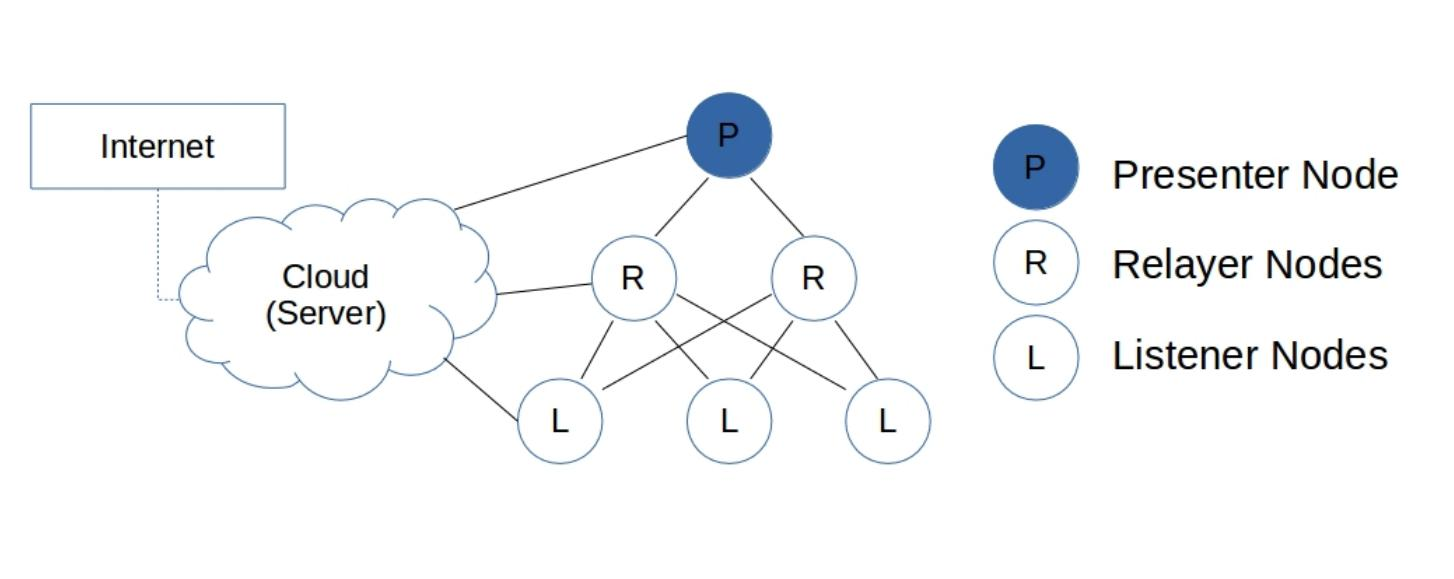
\includegraphics[width=0.5\textwidth]{figures/model1_test2.jpg}
  \caption{P2P-based Model for VoIP}
  %\vspace{-1in}
  \label{fig:mod1}
\end{figure}
There are four main types of components/nodes in the designed scenario, a
presenter, multiple relayers and listeners, and a remote cloud server.
In our application all the nodes are connected with the cloud server and
they do not need any kind of internet connection for transmitting voice through the network.
Each component can coordinate with one another in order to stream content such
as the voice or camera videos of the speaker, to the listeners in real-time. As
shown in Fig.~\ref{fig:mod1}, the network is organized in a hierarchical
architecture. The presenter will produce the streaming content from the
root node and broadcast it to the relayers and listeners, as well as to
the cloud servers for backup.

For example, one can think of the model as a lecture in real life. A presenter
is an instructor who gives the lecture in front of the room, and the
listeners are
students who are listening the lecture (can also be remote listening). When
a
presenter creates a presentation, the voice or videos being recorded will be
sent to both the child nodes and the remote cloud server so that the servers can
maintain a full copy for the streaming content in the presentation. All the
other nodes can passively receive the packets from the presenter.
%The relayers and cloud server are possible approaches the instructor adopts to
%pass on that voice stream.
%How well a student understand is not a good
%predictor of instructor’s capability; it largely depends on the media, that
%is, how well the instructor could transfer his thinking in a explanatory way.
%And that is where the cloud and relayers come into play.
There are different routes a voice packet can travel through. The
listeners receive voice packets through the relayers while the cloud server
can provide back-up services. If any of the listeners or relayers encounter a
data loss due to a bad network condition, the node can send requests to the
cloud server and retrieve the missing content. Once a relayer goes down,
the listeners will request the voice stream from the cloud. Presumably the
relayer will rejoin, and the system will reorganize to optimize in that case.
It is presumed that relayers are closer to the listeners, affording better
service due to locality and load distribution. The cloud will take
over
and serve as the main approach to deliver packets.
%Noted that only in simple cases where all attendees share the same role do
%relayers act as routers.
For a more complex scenario, where there are multiple roles for the listeners,
relayers act as filter and only forward packets to the designated attendees.

\begin{figure}[h!]
  \centering
      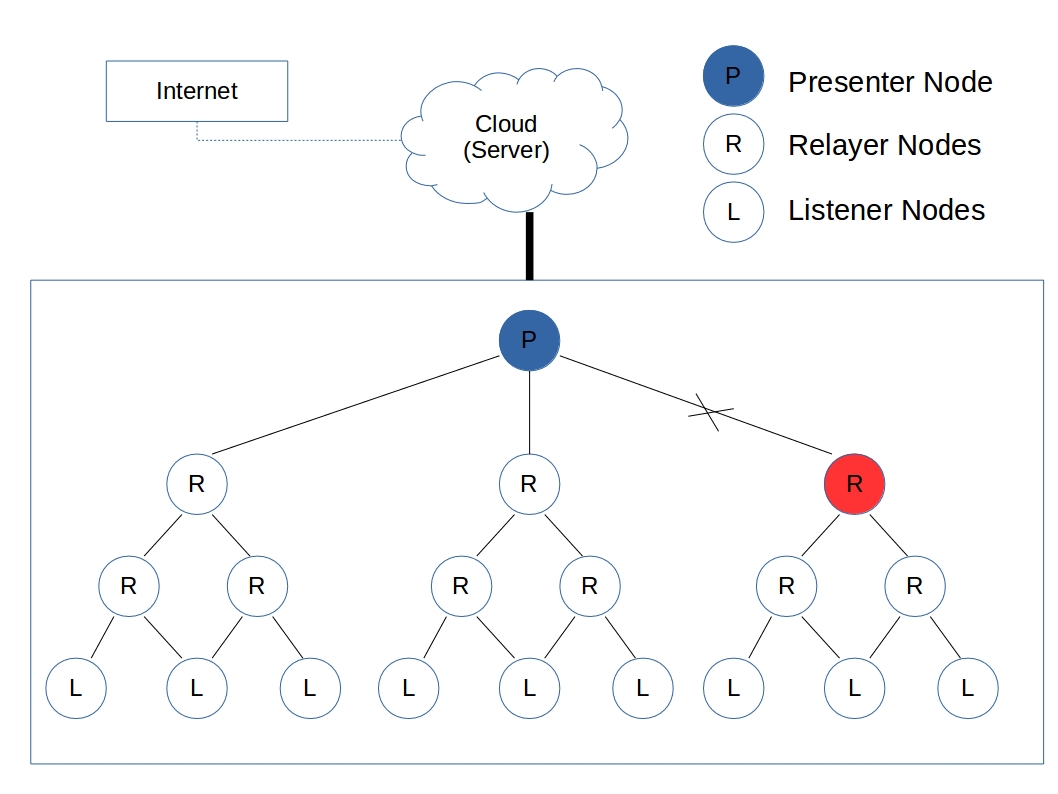
\includegraphics[width=0.5\textwidth]{figures/model2_test2.jpg}
  \caption{Relayers Become Presenters}
  \label{fig:mod2}
\end{figure}

However, this simple hierarchical architecture cannot be adaptable to
dynamic network changes and could experience an unbalanced network
traffic problem which could seriously reduce the quality of service and
experience. For example, Fig.~\ref{fig:mod2} shows that if a
high-level (near to the root) relayer suddenly leaves the network, all the
nodes lower than the relayer will not be able to receive the streaming content
any more, and thus the server will receive a large quality of requests from the
nodes which results in lossing the connection from the presenter. This will cause the server
bandwidth to be occupied by these nodes which will make the network flow
unbalanced. Also, the relayers among these nodes could lose their advantage in
passing the content to the listeners, as the listeners can already obtain the
requested packets from the cloud server and the bandwidth between the relayers
and the listeners is wasted.

Therefore, our proposed solution is to design a P2P-based
architecture among the relayers
and listeners. The server could act as the tracker in this scenario. Every node
will have to register with the server first when it joins in a presentation so
that the server will be aware of the network situation for each node. According
to the information the server receives from each node (including bandwith,
account information based on the future business model, etc.), some nodes will
be selected as relayers at different levels, while the other nodes will act as
the listeners (leaves) and establish connections with the relayers. The nodes
at the same level will be connected as well, to establish the P2P-based
architecture, as shown in Fig.~\ref{fig:mod3}.


\begin{figure}[h!]
  \centering
      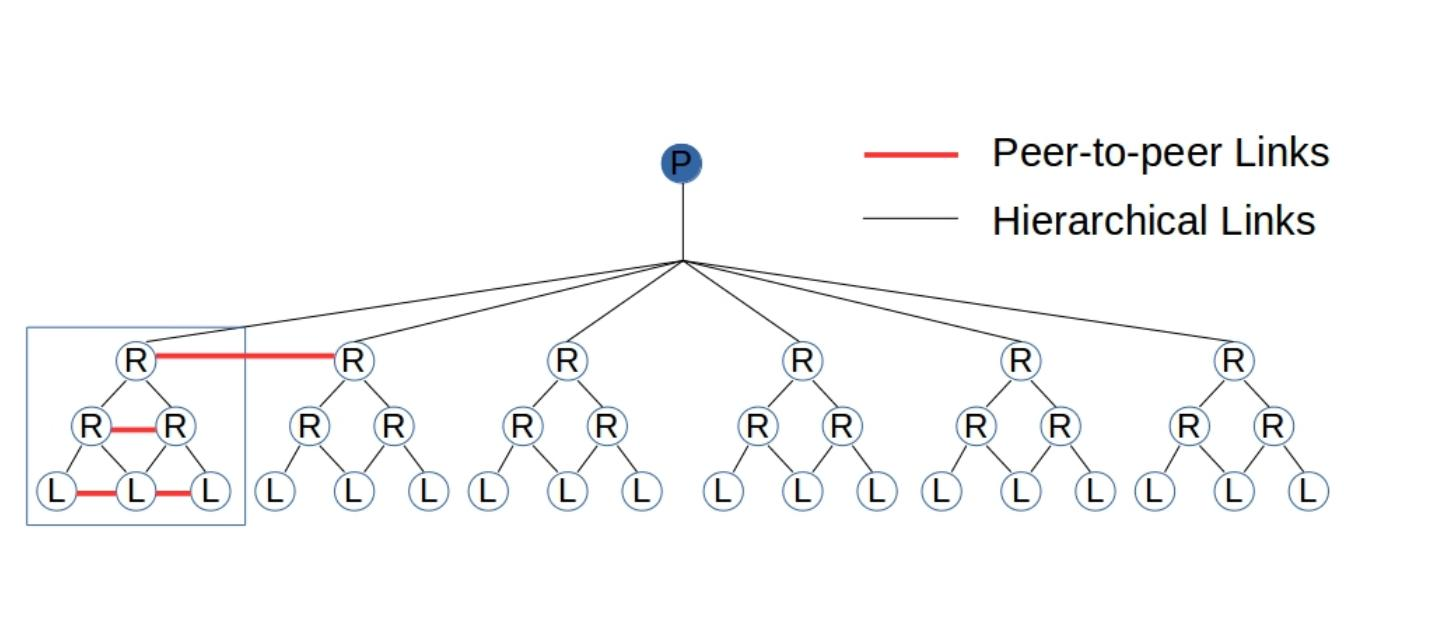
\includegraphics[width=0.5\textwidth]{figures/model3_test2.jpg}
  \caption{Relayers Become Presenters}
  \label{fig:mod3}
  \vspace{-0.15in}
\end{figure}


\begin{comment}
Besides, the concept of background channel will be applied for transmitting the
data in the background. Apart from the live channel which ensures the client to
have the presentation on live, there will also be a background channel to help
to upload or download previous missing data that make the data of the
presentation synchronized and completed in both server and client side while the
clients won’t even notice.
\end{comment}









%\section{The heuristic algorithm}\label{alg}
\section{Analysis and Case Study}
We used OMNeT++ as a simulation tool to explore the most
suitable model and algorithm for ThinkTogether. The study done by
Varga~\cite{A_OMNET_ESM01}
provides a brief introduction of OMNeT++, including Model Libraries, NED
language,
model structure. The paper also describes how to execute the simulation under a
powerful graphical user interface. Work done by Anggadjaja et
al.~\cite{EI_OMNET_ACT10}. features the
use of OMNeT++ based
simulation for a reliable point-to-point wireless transmission. The outcome could
provide inspiration for employing the P2P model in a wireless network. There
are several other papers~\cite{MM_OMNET_OMN08,XX_OMNET_ICQ12} explaining the
main infrastructure and
internal
design of OMNeT++.
%The team can gain overall understanding of the tool, through
%extensive papers above, and use OMNeT++ with efficiency and accuracy.

%Experimental data is the most scientific and objective way of verifying the
%efficiency of a particular network. There comes the simulation.
We evaluate several wireless and P2P frameworks~\cite{FBP_P2POVERLAY03},
such as MiXiM~\cite{XLL_MIXIM11}, OverSim~\cite{IBS_OVERSIM07}.
MiXiM is an OMNeT++ modeling framework created for mobile and fixed wireless
networks. MiXiM concentrates on the lower layers of the protocol stack, and offers
detailed models of radio wave propagation, interference estimation, radio transceiver
power consumption and wireless MAC protocols. OverSim is a flexible overlay network
simulation framework based on OMNeT++. OverSim includes several structured and
unstructured peer-to-peer protocols like Chord, Kademlia and Gia. Researchers can use
these protocols to run simulation for academic purpose as well as real world networks.

In our work, two network models will be built in order to observe the behavior
of data packets transferred in between the particular networks. One of the networking protocols
being used is Telnet, for which J. Postel et al~\cite{JJ_TEL83} provides the specification and
standards for using the protocol. This is a relatively old paper that was published in the early 1980s. The
paper draws a whole picture of the Telnet protocol from general consideration to
signal processing. Another protocol adopted is HTTP. There are wider
range of papers dedicated to HTTP. One of them is given by R Fielding~\cite{BJJH_HTTP1999}
, who provides a full-scaled overview, which can be used as a reference for modelling a network simulation.

%Multilayer Transmission

ThinkTogether is a communication application that contains multiple layers for
packet transmission. Data sent by each individual is handled differently. G.
Sekin et al~\cite{GF_COM00} provides an insight of how to manage multi
priority traffic in ATM network. The study is content-based video
objects. As the common characteristics shared between video stream and voice
stream, such as low tolerance in delay, jitter and packet loss. Unfortunately, there
is no evaluation involved in the paper, therefore the feasibility of the proposed
algorithm remains unknown.

After designing the model, we plan to create a working
network by creating a simulation using OMNeT++, as shown in Fig.~\ref{fig:sce}.
By creating this simulation we can have an idea of how the voice stream packets
are being transferred between the different nodes present in the network. Once
the simulation starts working for a basic scenario of just 2 leaf nodes, a
relayer and a cloud server, we will add more number of nodes to the simulation
and then analyse what changes are to be made to certain parameters of the
network so as to avoid any kind of latency and disturbance while transferring
the voice streams.

Presenters initialize services by sending voice packets to both relayers and
the cloud. Upon receiving the packets, the server stores them
locally and echoes back an acknowledgement. The services between presenter and
server is now finished. On the other side,
voice packets reach the relayer and will be directed to all attendees relayer
connects to, which is illustrated by \#6 and \#7 event in Fig.~\ref{fig:r_seq}.
Each attendees request the exact same voice data from the cloud.
Cloud handles the request by fetching corresponding data in server and sending
back the requested content. One can refer to events from \#11 to \#16 for
execution sequence details.



\section{Implementation: Data Distribution and Layers}

The simulation tests the efficiency in transferring voice data packets
with a fundamental model. This model lays the groundwork for future expansion,
and illustrates a simple way to consider a classroom scenario. The purpose of
the simulation is to investigate the feasibility, and more importantly, the efficiency of the
model. In the simulation, parameters such as packet drops, delay time, etc. are
collected and extracted to generate an output file for further analysis. The
output file is then used as
a foundation for performance analysis.


%In this paper our aim is to deploy a distributed the feature of voice
%streaming in the
%already developed application of Two Tall Totems called Think Together. In
%order to implement this feature we have
In our simulation of the model architecture, we use multiple nodes
as the leaf nodes in a network.
Then we also have some nodes that act as relayers in the network that will
transfer the voice stream from the presenter in the network to
the corresponding leaf nodes in the network. Along with all these nodes we also
have a cloud server which will act as a primary storage device for all the
voice streams that will be transmitted throughout the network. All the nodes will
have a direct link to the server so that if any of the leaf nodes (student
nodes in our scenario) want to retrieve any voice stream they can do so by
making a request to
the cloud server for that voice stream directly through the relayer (big node).

To simplify, we assume all the attendees are physically located in the same
classroom and they are subscribing to voice for the purpose of capturing the
information. This will eliminate potential influence caused by the difference
of
location, such as propagation delay. There are five components in the model:
presenter, relayer, cloud, server and attendee. Each component coordinates with
one another in order to offer recording services to attendees. There are two
test cases, one as a small-scaled network with two attendees, the other as a
slightly larger-scaled network with ten attendees. The simulation runs in HTTP net,
masking the lower level network layers such as TCP and IP.


%Model Taxonomy

Figure~\ref{fig:sce} shows the overall picture of the simulation model in a
small-scaled case. It shows the four main parts in the scenario: the sender (presenter), the receivers (attendees),
the relayers (mediators), and the cloud server (backup).

\begin{figure}[h!]
  \centering
    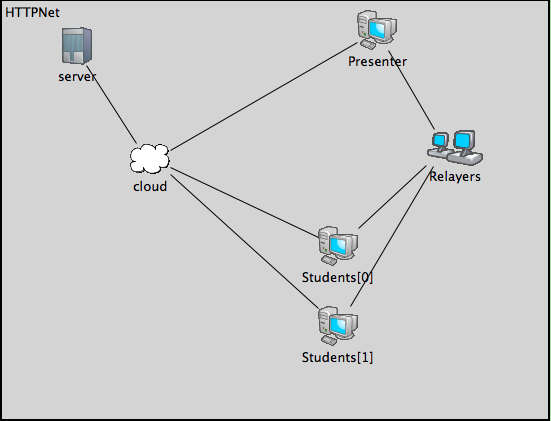
\includegraphics[width=0.5\textwidth]{figures/sce.png}
  \caption{Simulation in Omnet++}
  \label{fig:sce}
\end{figure}

Presenter is the starting point of the service. It does not rely on any outer
resource to trigger the sending process. Currently no packets other than
acknowledgement are sent to the presenters. In other words, one can view presenters
as a resource provider and there is no prerequisite for presenters to function.
There are two outgoing links connected to presenters. The one connected to
relayers is the main channel for delivering data. The one connected to cloud
transfers the same content, even though it is less demanding in terms of propagation
speed and processing time. A presenter sends voice packets to both links
simultaneously, and sets a timer for the next cycle.

The cloud server can be considered as a group in terms of services
purpose. They are both built to provide backup for attendees. There are two scenarios in
which attendees would need backup services. The first is when packets are lost by the
relayers and attendees will ask for complementary data from the cloud to ensure a
smooth stream. The second is when attendees are not able to attend
the class, but request a later review of that class. The server stores the
lectures in the format of voice stream and delivers it to attendees via cloud.
In this regard, the cloud is an interface between service providers and
receivers. In addition, once the network is scaled up to include multiple servers,
cloud acts as a coordinator that organizes the servers' actions.

The relayer acts as a router in this simple case simulation. Unlike servers,
the relayer
does
not store voice data, therefore all the attendees can not request data from the relayer
later on. It should be noted that this primary function is not yet implemented,
and will be
addressed later in the future model.

Attendees are students in the diagram. They receive voice packets from
presenters, regularly through relayers. It should be noted that attendees will
not send
acknowledgement back to presenters. When the network between relayers and
attendees are down, or for some reason, packets are lost in the regular
transmission routes, attendees will request the data from the server. The
target
users of the ThinkTogether application are attendees and presenters.
%Execution Sequence:

To collect data from multiple cycles, we set a timer for both presenter and
attendees based on an exponential distribution. After sending the voice
packets,
the presenter will create a timer that controls how long before the next cycle,
namely, the next time it starts sending the packets. The duration of the timer
is based on a exponential function, which allows random distribution in sending
packets. The same principle applies to the rate of sending request from attendees.
There is also a timer created by attendee that controls the rate of sending
requests to the cloud. In real life, an attendee will need the complementary data from cloud
only when the relayers fail to deliver it. However, in order to fully evaluate the
function, in the simulation we configure an attendee to request voice data from
the cloud whether the relayers go down or not.

\begin{figure}[h!]
  \centering
    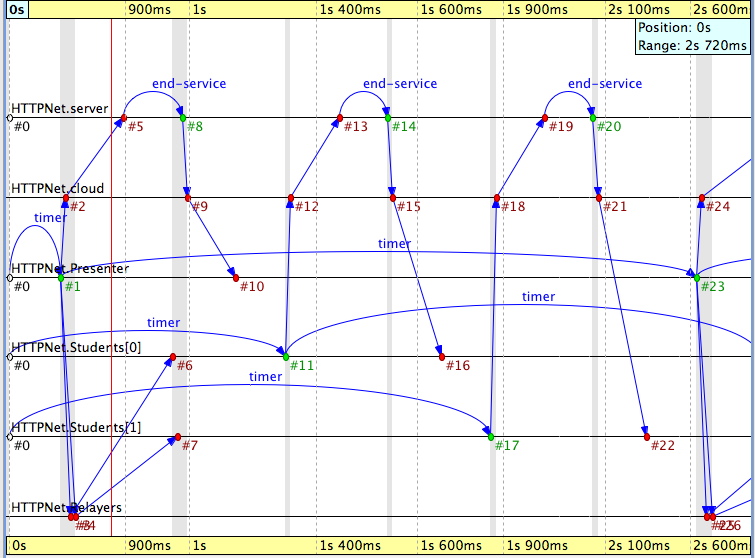
\includegraphics[width=0.45\textwidth]{figures/r_seq.png}
  \caption{Events in Time Sequence}
  \label{fig:r_seq}
  \vspace{-0.2in}
\end{figure}

The execution sequence is illustrated in Fig.~\ref{fig:r_seq}. It is a log file
generated by running small-scaled cases.

%\section{Deployment: Distributed Cloud}




%\section{Performance Evaluation}\label{simu}
%\section{Performance Evaluation}

%\section{Conclusion and Further Work}\label{conclu}
\section{Conclusions and Future Work} 
In this paper, we have initiate a model which decentralizes the location of 
shared content within a peer-to-peer structure for a CSCW application (VoIP). 
As a part of future work, we aim to extend this application for people who can 
download the voice stream from the presentation remotely in real-time. We also 
aim to use a hierarchical structure for the network which will help the 
different nodes present in the network to change their roles during the 
presentation at any time. Once the application is working perfectly for a 
limited number of users we aim to extend this application in a way so that it 
can be used for any number of users without having any storage issues, any 
disruption in the voice streaming or any bandwidth issues in the network by 
adding large number of users to the presentation. Another thing that we will 
take care of in the future is that if any of the relayer nodes fails then all 
the leaf nodes linked to that relayer will be dynamically transferred to 
another relayer. New schemes will be developed to guarantee that these dynamic 
changes will not significantly reduce the network performance, as well as to 
keep a balanced traffic flow with the optimal bandwidth utilization.

%\input{appendix}


\bibliographystyle{plain}
\begin{thebibliography}{10}

\begin{comment}
\bibitem{IEEEhowto:kopka}
H.~Kopka and P.~W. Daly, \emph{A Guide to \LaTeX}, 3rd~ed.\hskip 1em plus
  0.5em minus 0.4em\relax Harlow, England: Addison-Wesley, 1999.

\bibitem{sample}
\newblock ``Efficient user-assisted content distribution over
information-centric
  network,''
\newblock In {\em Proc. IFIP Networking Conference}, pp. 1--12, 2012.
\end{comment}

%ref 00
\bibitem{XG_P2P_INFO04}
X.~Yang, and G.~Veciana,
\newblock ``Service capacity of peer to peer networks,''
\newblock In {\em IEEE Proc. of the Twenty-third Annual Joint Conference on
Computer and Communications (INFOCOM)}, pp. 2242--2252, 2004.

%ref 16
\bibitem{A_OMNET_ESM01}
A.~Varga,
\newblock ``The OMNeT++ discrete event simulation system,''
\newblock In {\em Proc. of the European simulation multiconference (ESM)},
9(185), 2001.

%ref 01
\bibitem{HS_VoIP_ICTC10}
H.~Wook and S.~Kang,
\newblock ``Design and implementation of SIP-based mobile VoIP
application for multiple smartphone OS,''
\newblock In {\em Proc. Information and Communication
Technology Convergence (ICTC)}, pp. 565--568, 2010.

%ref 02
\bibitem{HSR_VoIP_TVT07}
H.~Fathi, S.~S.~Chakraborty, and R.~Prasad,
\newblock ``Optimization of Mobile IPv6-Based Handovers to Support VoIP Services
in Wireless Heterogeneous Networks,''
\newblock In {\em IEEE Transactions on Vehicular Technology}, 56(1):260--270,
2007. doi: 10.1109/TVT.2006.883806.

%ref 03
\bibitem{HYS_VoIP_COM00}
H.~C.~Rao, Y.~Lin, S.~Cho,
\newblock ``iGSM: VoIP service for mobile networks,''
\newblock In {\em IEEE Communications Magazine}, 38(4):62--69, 2000.
 doi: 10.1109/35.833558.

%ref 04
\bibitem{MRSR_VoIP_COM08}
M.~Fong, R.~Novak, S.~Mcbeath, and R.~Srinivasan,
\newblock ``Improved VoIP capacity in mobile WiMAX systems using persistent
resource allocation,''
\newblock In {\em IEEE Communications Magazine}, 46(10):50--57, 2008.
doi: 10.1109/MCOM.2008.4644119.

%ref 05
\bibitem{OR_VoIP_PMC03}
O.~Komolafe and R.~Gardner,
\newblock ``Aggregation of VoIP streams in a 3G mobile network: a teletraffic
perspective,''
\newblock In {\em Proc. Personal Mobile Communications Conference}, pp.
545--549, 2003. doi: 10.1049/cp:20030314.

%ref 06
\bibitem{YRAP_VoIP_MSYS07}
Y.~Agarwal, R.~Chandra, A.~Wolman, P.~Bahl, K.~Chin, and R.~Gupta,
\newblock ``Wireless wakeups revisited: energy management for voip over WiFi
smartphones,''
\newblock In {\em ACM Proc. of the 5th international conference on Mobile
systems, applications and services (MobiSys)}, pp. 179--191, 2007.
doi=10.1145/1247660.1247682.

%ref 07
\bibitem{WPY_VoIP_SYS11}
W.~Chen, P.~Lin, and Y.~Lin,
\newblock ``Real-Time VoIP Quality Measurement for Mobile Devices,''
\newblock In {\em IEEE Systems Journal}, 5(4):538--544, 2011.
doi: 10.1109/JSYST.2011.2165604.

%ref 08
\bibitem{DHMS_WiMAX_WOW08}
D.~Kim, H.~Cai, M.~Na, S.~Choi,
\newblock ``Performance measurement over Mobile WiMAX/IEEE 802.16e network,''
\newblock In {\em International Symposium on World of Wireless, Mobile and
Multimedia Networks (WoWMoM)}, 1(8):23--26, June 2008.
doi: 10.1109/WOWMOM.2008.4594817.

%ref 09
\bibitem{SMPM_VoIP_ICAESM12}
S.~Sundar, M.~K.~Kumar, P.~Selvinpremkumar, and M.~Chinnadurai,
\newblock ``Voice over IP via Bluetooth/Wi-Fi Peer to Peer,''
\newblock In {\em International Conference on Advances in Engineering, Science
and Management (ICAESM)}, pp. 828--837, March 2012.

%ref 10
\bibitem{GWA_P2P_VoIP_ICWMC10}
G.~Kbar, W.~Mansoor, A.~Naim,
\newblock ``Voice over IP Mobile Telephony Using WiFi P2P,''
\newblock In {\em the 6th International Conference on Wireless and Mobile
Communications (ICWMC)}, pp. 268--273, September 2010.
doi: 10.1109/ICWMC.2010.97.

%ref 11
\bibitem{GCXZ_P2PVoIP_MTA13}
G.~Wang, C.~Zhang, X.~Qiu, and Z.~Zeng,
\newblock ``An efficient relay node selection scheme to improve the performance
of P2P-based VoIP applications in Chinese internet,''
\newblock In {\em Multimedia Tools and Applications}, 64(3):599--625, 2013.
doi: 10.1007/s11042-011-0952-5.

%ref 12
\bibitem{SN_Skype_CIST05}
S.~Guha and N.~Daswani,
\newblock ``An Experimental Study of the Skype Peer-to-Peer VoIP System,''
\newblock In {\em Computing and Information Science Technical
Reports}, 2005.

%ref 13
\bibitem{TA_Skype_COMPNET08}
T.~Hoßfeld and A.~Binzenhöfer,
\newblock ``Analysis of Skype VoIP traffic in UMTS: End-to-end QoS and QoE
measurements,''
\newblock In {\em Computer Networks}, 52(3):650--666, 2008.
doi: 10.1016/j.comnet.2007.10.008.

%ref 14
\bibitem{SH_Skype_INFO06}
S.~A.~Baset, and H.~Schulzrinne,
\newblock ``An analysis of the skype peer-to-peer internet telephony protocol,''
\newblock In {\em IEEE Proc. of the 25th IEEE International Conference
on Computer Communications (INFOCOM)}, pp.1--11, April 2006.
doi: 10.1109/INFOCOM.2006.312.


%ref 15
\bibitem{JSPS_USPatent05}
J.~Fobert, S.~Navaratnam, P.~J.~Dagert, and S.~J.~McKinnon,
\newblock ``Client-server network for managing Internet protocol
voice packets''
\newblock U.S. Patent No. 6,853,713, February 2005.


%ref 17
\bibitem{EI_OMNET_ACT10}
E.~Anggadjaja, and I.~McLoughlin,
\newblock ``Point-to-point OMNeT++ based simulation of reliable transmission
using realistic segmentation and reassembly with error control,''
\newblock In {\em IEEE second International Conference on Advances in
Computing, Control and Telecommunication Technologies (ACT)}, pp. 125--128,
2010.

%ref 18
\bibitem{MM_OMNET_OMN08}
M.~Bohge, and M.~Renwanz,
\newblock ``A realistic VoIP traffic generation and evaluation tool for
OMNeT++,''
\newblock In {\em Proc. of the 1st International Workshop on OMNeT++},
March 2008.

%ref 19
\bibitem{XX_OMNET_ICQ12}
X.~Qing, and X.~Ren,
\newblock ``Research of routing protocols simulation for wireless sensor
networks based on OMNeT++,''
\newblock In {\em IEEE International Conference on Quality, Reliability, Risk,
Maintenance, and Safety Engineering (ICQR2MSE)}, pp. 79--82, June 2012.

%ref 20
\bibitem{FBP_P2POVERLAY03}
F.~Dabek, B.~Zhao, P.~Druschel, J.~Kubiatowicz, and I.~Stoica, 
\newblock ``Towards a common API for structured peer-to-peer overlays,'' 
\newblock In {\em Proceedings of the 2nd International Workshop on Peer-toPeer Systems (IPTPS)}, pp. 33--44, 2003.

%ref 21
\bibitem{XLL_MIXIM11}
X.~Li, L.~Wang, L~Liu, X.~Hu, F.~Xu and J.~Chen, 
\newblock ``OMNeT++ and Mixim-based protocol simulator for satellite network,'' 
\newblock In {\em IEEE Aerospace Conference}, pp. 1--9, 2011.

%ref 22
\bibitem{IBS_OVERSIM07}
I.~Baumgart, B.~Heep, S.~Krause,
\newblock ``OverSim: A Flexible Overlay Network Simulation Framework,''
\newblock In {\em IEEE Global Internet Symposium}, pp. 79--84, 2007.

%ref 23
\bibitem{JJ_TEL83}
J.~Postel, and J.~K.~Reynolds,
\newblock ``Telnet protocol specification,'' 1983.

%ref 24
\bibitem{BJJH_HTTP1999}
R.~Fielding, J.~Gettys, J.~Mogul, H.~Frystyk, L.~Masinter, P.~Leach, and T.~
Berners-Lee,
\newblock ``Hypertext transfer protocol–HTTP/1.1,'' 1999.

%ref 25
\bibitem{GF_COM00}
G.~Seckin, and F.~Golshani,
\newblock ``Real-time transmission of multilayer video over ATM networks,''
\newblock In {\em Computer Communications}, 23(10):962--974, 2000.


\end{thebibliography}

%\bibliography{pacrim15}


\end{document}
